\documentclass{article}
\usepackage[paperwidth=21.0cm,paperheight=9cm,margin=0cm,noheadfoot]{geometry}
\usepackage{amsmath,amssymb}
\usepackage{tikz}
\usetikzlibrary{arrows.meta,positioning,calc,backgrounds}
\usepackage{xcolor}
\usepackage[T1]{fontenc}
\usepackage{lmodern}
\usepackage{tgheros}
\usepackage{sansmath}
\renewcommand{\familydefault}{\sfdefault}
\sansmath
\pagestyle{empty}
\setlength{\parindent}{0pt}

% === Colors ===
\definecolor{deepblue}{HTML}{1A5276}
\definecolor{midblue}{HTML}{2980B9}
\definecolor{lightblue}{HTML}{AED6F1}
\definecolor{lightblue2}{HTML}{D4E6F1}

\definecolor{deepgreen}{HTML}{1E6B3A}
\definecolor{midgreen}{HTML}{27AE60}
\definecolor{lightgreen}{HTML}{A9DFBF}

\definecolor{coralpink}{HTML}{E74C3C}
\definecolor{deepgray}{HTML}{2C3E50}
\definecolor{midgray}{HTML}{7F8C8D}
\definecolor{panelbg}{HTML}{FAFCFE}

\begin{document}
\vspace*{0pt}\noindent
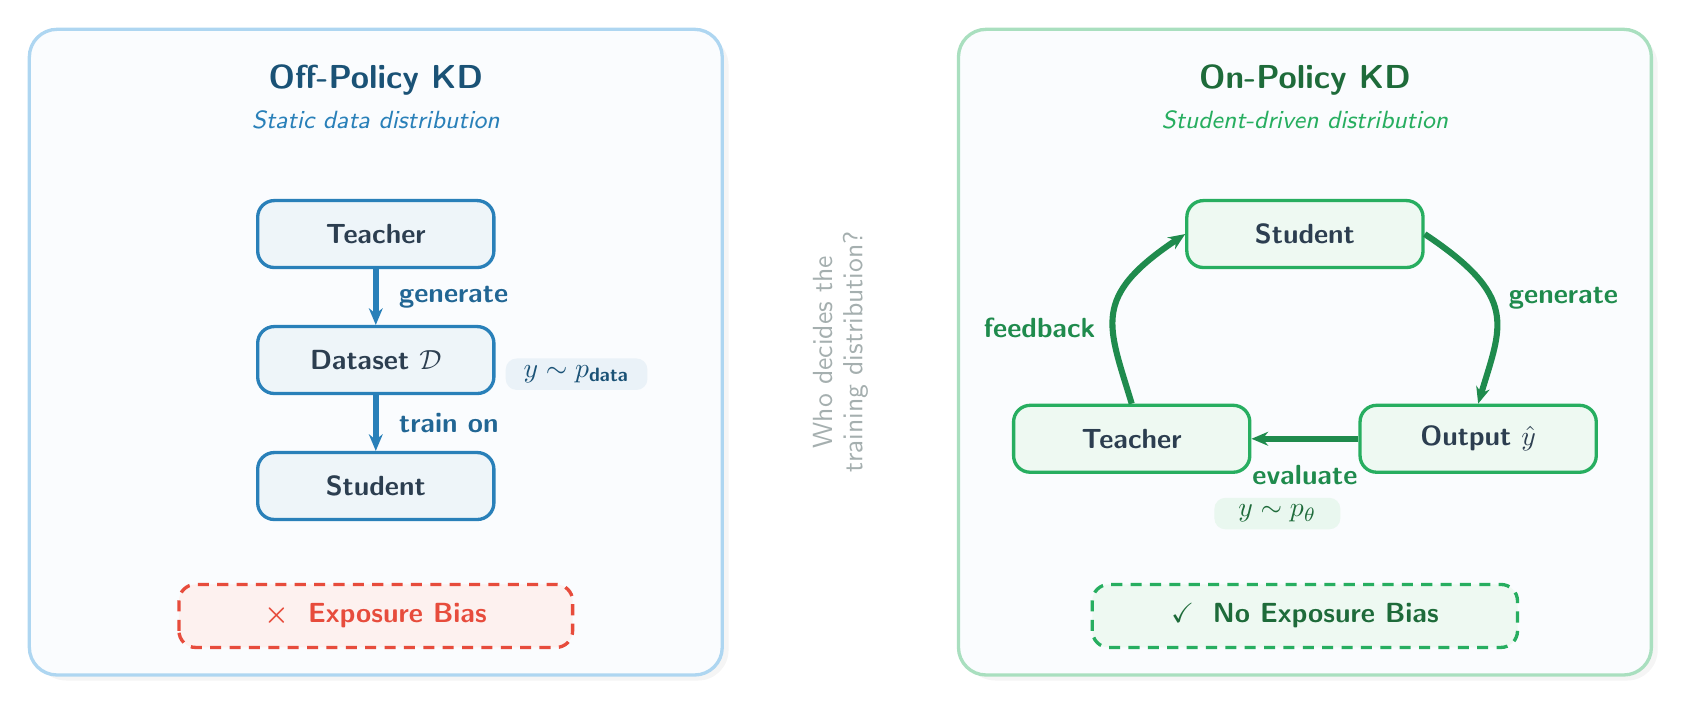
\begin{tikzpicture}[
    >=Stealth,
    nodebox/.style={
      draw=#1, line width=1.2pt, rounded corners=6pt,
      fill=#1!8,
      font=\normalsize\bfseries, text=deepgray,
      minimum width=3.0cm, minimum height=0.85cm,
      text centered, inner sep=5pt,
    },
    arr/.style={-{Stealth[length=6pt,width=5pt]}, line width=2.2pt, #1},
    lbl/.style={font=\normalsize\bfseries, #1},
  ]

  % =================== LEFT PANEL: Off-Policy KD ===================
  % Shadow
  \fill[black, opacity=0.04, rounded corners=11pt] (0.08, -0.07) rectangle (8.88, 8.13);
  % Background
  \fill[panelbg, rounded corners=10pt] (0, 0) rectangle (8.8, 8.2);
  \draw[lightblue, line width=1.2pt, rounded corners=10pt] (0, 0) rectangle (8.8, 8.2);

  % Title
  \node[font=\large\bfseries, deepblue] at (4.4, 7.55) {Off-Policy KD};
  \node[font=\small\itshape, midblue] at (4.4, 7.05) {Static data distribution};

  % Nodes — vertical flow (tighter spacing)
  \node[nodebox=midblue] (T1) at (4.4, 5.6) {Teacher};
  \node[nodebox=midblue] (D1) at (4.4, 4.0) {Dataset $\mathcal{D}$};
  \node[nodebox=midblue] (S1) at (4.4, 2.4) {Student};

  % Arrows with labels
  \draw[arr=midblue] (T1) -- (D1)
    node[midway, right, lbl=midblue!80!black, xshift=4pt] {generate};
  \draw[arr=midblue] (D1) -- (S1)
    node[midway, right, lbl=midblue!80!black, xshift=4pt] {train on};

  % Distribution badge — flush right of Dataset
  \fill[midblue!10, rounded corners=4pt] (6.05, 3.62) rectangle (7.85, 4.02);
  \node[font=\normalsize\bfseries, deepblue] at (6.95, 3.82) {$y \sim p_{\text{data}}$};

  % Warning badge — Exposure Bias
  \fill[coralpink!8, rounded corners=6pt] (1.9, 0.35) rectangle (6.9, 1.15);
  \draw[coralpink, line width=1.2pt, rounded corners=6pt, dash pattern=on 4pt off 3pt] (1.9, 0.35) rectangle (6.9, 1.15);
  \node[font=\normalsize\bfseries, coralpink] at (4.4, 0.75) {$\boldsymbol{\times}$\; Exposure Bias};

  % =================== CENTER DIVIDER ===================
  \node[font=\normalsize, midgray!70, rotate=90, text width=4.0cm, align=center] at (10.3, 4.1)
    {Who decides the\\[-1pt]training distribution?};

  % =================== RIGHT PANEL: On-Policy KD ===================
  % Shadow
  \fill[black, opacity=0.04, rounded corners=11pt] (11.88, -0.07) rectangle (20.68, 8.13);
  % Background
  \fill[panelbg, rounded corners=10pt] (11.8, 0) rectangle (20.6, 8.2);
  \draw[lightgreen, line width=1.2pt, rounded corners=10pt] (11.8, 0) rectangle (20.6, 8.2);

  % Title
  \node[font=\large\bfseries, deepgreen] at (16.2, 7.55) {On-Policy KD};
  \node[font=\small\itshape, midgreen] at (16.2, 7.05) {Student-driven distribution};

  % Nodes — triangle layout (Student top, Teacher bottom-left, Output bottom-right)
  \node[nodebox=midgreen] (S2) at (16.2, 5.6) {Student};
  \node[nodebox=midgreen] (T2) at (14.0, 3.0) {Teacher};
  \node[nodebox=midgreen] (O2) at (18.4, 3.0) {Output $\hat{y}$};

  % Cycle arrows
  % Student → Output (generate): right side
  \draw[arr=midgreen!80!black] (S2.east) .. controls ++(1.2,-0.8) and ++(0.3,1.0) .. (O2.north)
    node[pos=0.4, right, lbl=midgreen!80!black, xshift=2pt] {generate};
  % Output → Teacher (evaluate): bottom
  \draw[arr=midgreen!80!black] (O2.west) -- (T2.east)
    node[midway, below, lbl=midgreen!80!black, yshift=-5pt] {evaluate};
  % Teacher → Student (feedback): left side
  \draw[arr=midgreen!80!black] (T2.north) .. controls ++(-0.3,1.0) and ++(-1.2,-0.8) .. (S2.west)
    node[pos=0.4, left, lbl=midgreen!80!black, xshift=-2pt] {feedback};

  % Distribution badge
  \fill[midgreen!10, rounded corners=4pt] (15.05, 1.85) rectangle (16.65, 2.25);
  \node[font=\normalsize\bfseries, deepgreen] at (15.85, 2.05) {$y \sim p_\theta$};

  % Success badge — No Exposure Bias
  \fill[midgreen!8, rounded corners=6pt] (13.5, 0.35) rectangle (18.9, 1.15);
  \draw[midgreen, line width=1.2pt, rounded corners=6pt, dash pattern=on 4pt off 3pt] (13.5, 0.35) rectangle (18.9, 1.15);
  \node[font=\normalsize\bfseries, deepgreen] at (16.2, 0.75) {$\boldsymbol{\checkmark}$\; No Exposure Bias};

\end{tikzpicture}
\end{document}
